\documentclass[oneside]{book}

\setcounter{secnumdepth}{4}

\setcounter{tocdepth}{4}

\usepackage{graphicx}



\usepackage{geometry}
\usepackage{listings}
\lstdefinestyle{lsstyle}{
	basicstyle=\ttfamily,
	basicstyle=\small,
	captionpos=b
}


\usepackage[bottom]{footmisc}

\usepackage{varwidth}

\lstset{style=lsstyle}

\usepackage{amsmath,systeme}

\DeclareMathOperator*{\argmax}{arg\,max}

\usepackage{verbatim}

\usepackage{courier}

\usepackage{hyperref}

\usepackage{url}

\geometry{a4paper}



\begin{document}



\begin{titlepage} 
	\noindent
	\begin{minipage}[t]{0.19\textwidth}
		\vspace{-4mm}{
\includegraphics[scale=1.15]{logo_unimib.pdf}}
	\end{minipage}
	\begin{minipage}[t]{0.81\textwidth}
	{
	{\textsc{Università degli Studi di Milano - Bicocca}} \\
	\textbf{Scuola di Scienze} \\
	\textbf{Dipartimento di Informatica, Sistemistica e Comunicazione} \\
	\textbf{Corso di laurea in Informatica} \\
	\par
	}
	\end{minipage}
	\vspace{40mm}
	
	\begin{center}{\LARGE{\textbf{Enhancing irony detection with affective information}\par}}
	\end{center}        
	\vspace{50mm}
	\noindent
	{\large \textbf{Relatore:} Prof. Elisabetta Fersini} \\        
	\vspace{15mm}
	\begin{flushright}
		{\large \textbf{Relazione della prova finale di:}} \\
		\large{Gianluca Giudice} \\
		\large{Matricola 830694} 
	\end{flushright}
	\vspace{20mm}
	\begin{center}
		{\large{Anno Accademico 2019-2020}}
	\end{center}
\end{titlepage}
	
	

\tableofcontents

% 3 PAGINE
\chapter*{Introduzione}

\section*{Descrizione del problema}

La sentiment analysis è un campo dell'elaborazione del linguaggio naturale (NLP) che si occupa di costruire sistemi per l'analisi di un testo, ha il fine di identificare e classificare l'informazione come il sentimento e l'opinione espressa nello stesso. Si basa sui principali metodi di linguistica computazionale e di analisi testuale. L'analisi del sentiment è utilizzata in molteplici settori: dalla politica ai mercati azionari, dal marketing alla comunicazione, dall'analisi dei social media alla valutazione delle preferenze del consumatore. 

Il riconoscimento automatico dell'ironia nei contenuti generati da utenti, è uno dei compiti più complessi per quanto riguarda l'elaborazione del linguaggio naturale. Tuttavia è di fondamentale importanza per tutti i sistemi di sentiment analysis, in quanto facendo uso dell'ironia è possibile invertire completamente la polarità di una propria opinione, facendola passare da positiva a negativa e viceversa.
Diventa pertanto cruciale sviluppare dei sistemi di sentiment analysis che sono consapevoli del fenomeno e in grado di riconoscerlo.

L'ironia è un tema studiato in diverse discipline, come la linguistica, filosofia e psicologia, ma è difficile da definire formalmente, soprattutto per questo motivo ne è difficile il riconoscimento. Nonostante ciò ci sono basi teoriche che suggeriscono il ruolo importante della sfera emozionale nell'uso dell'ironia, quindi un fattore chiave per riconoscerlo. Con questo si intende anche un uso indiretto e non esplicito del carico emotivo in ciò che si vuole comunicare.

I social netowork in generale, e twitter nello specifico, sono ampiamente utilizzati come fonte di informazione per comprendere la web reputation di un brand, perciò si prestano bene per la sperimentazione di modelli computazionali per il riconoscimento dell'ironia, essendo di fatti una grande risorsa per quanto riguarda i dati testuali generati da utenti.


\section*{Approccio al problema}
Parlare QUI di machine learning e di intelligenza artificiale




Si può considerare il riconoscimento dell'ironia come un problema di classificazione. Una frase potrà quindi essere classificata come appartenente alla classe ironica o non ironica. Si noti che per come viene approcciato il problema, l'ironia è considerata al pari del sarcasmo.

Come già detto, twitter è una risorsa che fornisce moltissimi contenuti generati da utenti. Viene sfruttato questo aspetto per creare dei modelli supervisionati di machine learning in grado di apprendere dai dati con lo scopo di riconoscere l'ironia nel testo.

Il codice sviluppato è in questo repo:
www.github



\section*{Sintesi dei risultati}
Devo mettere le tabelle i grafici? Quanto deve essere sintetico?


\chapter{Stato dell'arte}

\section{Approccio supervisionato}

\section{Approccio semi supervisionato}

\section{Approccio non supervisionato}


\chapter{Sistema realizzato}

\section{Descrizione del sistema proposto}
Partendo dai dati a disposizione si utilizzano delle tecniche di preprocessing che consistono nel pulire il testo di partenza e prepararlo per essere dato in input ai vari classificatori. Inoltre si estraggono delle features da ogni messaggio, le quali più sono discriminanti nel riconoscimento dell'ironia, meglio distinguono la classe di appartenenza.

Il dataset viene diviso in due parti: training set e test set. La prima ha dimensione decisamente maggiore e viene utilizzata per far apprendere uno specifico classificate, l'altra per testarlo. Questo è importante in quanto un determinato modello dovrà riconoscere l'ironia in un generico documento e non solo tra quelli a disposizione. Si noti che entrambe le porzioni sono composte sia dal testo già codificato e processato che le features estratte, hanno solo scopi diversi quando si tratta di creare il classificatore. 

Vengono quindi creati vari modelli supervisionati di machine learning fornendo in input il dataset di training. Avendo costruito più classificatori che utilizzano diversi algoritmi per apprendere dai dati, è possibile confrontarne le performance per valutare il migliore tra tutti, ovvero quello che meglio distingue tra documenti ironici e non ironici.

\begin{figure}
	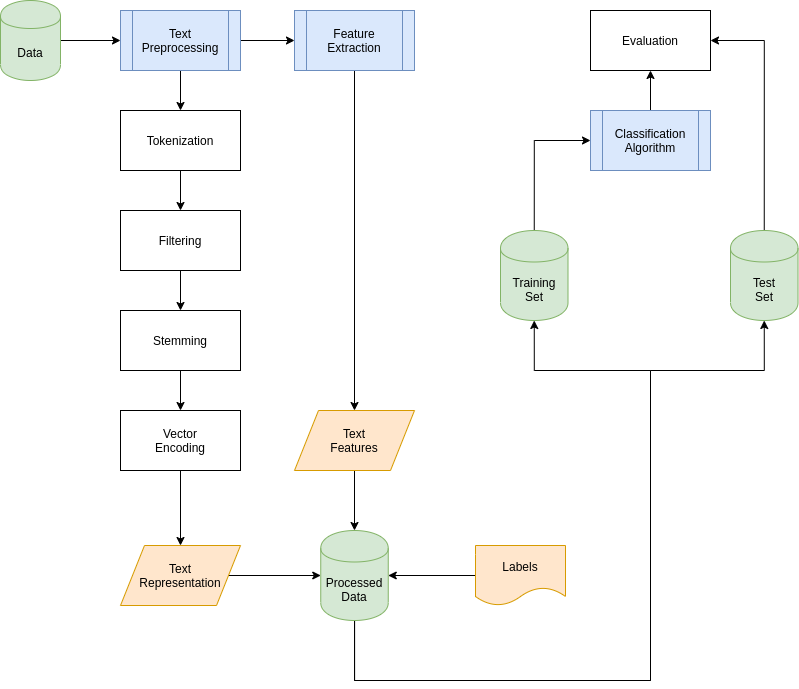
\includegraphics[width=\linewidth]{assets/Workflow.png}
	\caption{Workflow.}
	\label{fig:workflow}
\end{figure}


\clearpage

\section{Dati in input}

Per procedere con la costruzione di modelli supervisionati per il riconoscimento dell'ironia, è necessaria una collezione di testi (in questo caso tweet) che insieme alle relative etichette associate ad ogni documento, costituisce il dataset. Questo aspetto è cruciale in quanto, una volta essere stati opportunamente processati, saranno proprio questi i dati forniti in input al classificatore, e hanno lo scopo di farlo apprendere e quindi successivamente riconoscere l'ironia in testi che non ha mai visto prima.


\begin{table}[h!]
	\centering
	\begin{tabular}[t]{lr}
		\hline
		\textbf{Tweet} & \textbf{Label assocaita}\\
		\hline
		Lorem ipsum dolor sit amet, consectetur adipiscing elit & ironico     \\
		Cras ornare turpis ut odio finibus, viverra porta felis lobortis & ironico \\
		Suspendisse in ex a felis porta convallis & non ironico \\
		Nam laoreet, lacus at ullamcorper iaculis, id interdum nisl elit nec elit. & non ironico \\
		
		\hline
	\end{tabular}
	\caption{Esempio di dataset a disposizione.}
\end{table}%




\section{Rappresentazione del testo}
Il corpora a disposizione è definito "crudo" e non può essere direttamente utilizzato la fase di training. Prima è necessario codificare il testo per ottenere una rappresentazione numerica da dare in input ad un algoritmo di classificazione per la fase di training e test. A questo scopo sono state utilizzate due diverse tecniche

\subsection{Rappresentazione Bag-of-word}
La prima tecnica di rappresentazione utilizzata è boolean bag-of-words.
Il testo viene codificato come una matrice booleana costituita dai documenti sulle righe e i tokens sulle colonne. I tokens sono tutte quelle parole appartenenti ad un dizionario costruito a partire dal corpora, tutte le operazioni eseguite sono spiegate di seguito.

\subsubsection{Tokenization}
La tokenizzazione è un passo preliminare per l'elaborazione computazionale del testo. Tokenizzare vuol dire dividere le sequenze di caratteri in unità minime di analisi dette "token". Un approccio potrebbe essere considerare un token come una sequenza di caratteri delimitata da spazi, tuttavia una tale definizione lascia spazio a numerose eccezzione, come ad esempio la presenza di punteggiatura. Per questa operaziona viene pertanto utilizzata la libreria
nltkl\footnote{Natural Language Toolkit: \url{www.nltk.org}} in grado di gestire correttamente tutti questi casi limite, oltre a poter sfruttare una Twitter-aware tokenization adattandosi quindi bene al dominio in questione.

\begin{figure}[!h]
	\centering
	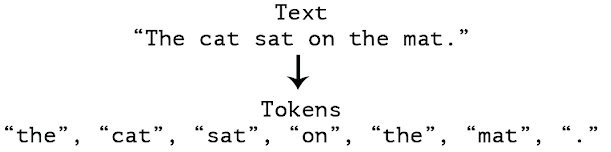
\includegraphics[width=9cm]{assets/text-to-tokens.jpg}
	\caption{Text tokenization.}
	\label{fig:tokenization}
\end{figure}


\pagebreak

I vari tokens estratti vengono convertiti in lowercase e sono considerati validi solo se in match con il pattern regex \texttt{[a-z]+}. Così facendo non si considerano gli hashtag, la punteggiatura, le emoji e tutto ciò che non è considerato una parola. Si noti che potrebbero verificarsi casi in cui lo stesso token è presente in documenti diversi, questo è ragionevole in quanto le stesse parole possono essere presenti in tweet diversi.


Il risultato ottenuto è una lista di tokens validi contenuti in ogni tweet:

\begin{table}[h!]
	\centering
	\begin{tabular}[t]{l|l}
		\hline
		\textbf{Tweet} & \textbf{Tokens lowercase}\\
		\hline
		Lorem ipsum dolor sit amet, consectetur adipiscing elit				& [$t_1$, $t_2$, $t_3$, $t_4$, $t_5$] \\
		Cras ornare turpis ut odio finibus, viverra porta felis lobortis 	& [$t_6$, $t_7$, $t_1$, $t_8$, $t_9$, $t_4$] \\
		Suspendisse in ex a felis porta convallis							& [$t_{10}$, $t_6$, $t_{11}$, $t_{12}$] \\
		Nam laoreet, lacus at ullamcorper iaculis.							& [$t_{13}$, $t_{14}$, $t_8$, $t_{15}$]\\
		
		\hline
	\end{tabular}
	\caption{Esempio di tokens associati ad ogni tweet.}
\end{table}

Da qui si crea l'insieme di tokens univoci.

\subsubsection{Filtering}
L'insieme di termini univoci ottenuto è filtrato in base ai seguenti criteri:
\begin{itemize}
	\item \textbf{Occorrenza minimia} fissato valore di threshold
		
		Viene fissato un valore di soglia (Es. 10) e si scartano tutte quelle parole che compaiono tra tutti i testi meno del valore scelto. 
	\item \textbf{Stopwords + RT}
	
		Vengono scartate tutte le parole più comuni che sono generalmente presenti in una frase. Queste sono un insieme predefinito contenente parole come gli articoli, proposizioni, pronomi e verbi ausiliari.
		
		Es: $\{a,\ the,\ of,\ is,\ into,\ it,\ ...\}$
		
		Dato il dominio preso in considerazione, è possibile che un utente compia l'operazione di ReTweet. Questo è codificato nei messaggi dall'abbreviazione \emph{"rt"}. Non ritenendolo un aspetto rilevante per il riconoscimento dell'ironia, viene anch'essa considerata una stopwords, e di conseguenza non trattato come token valido.
	
		
	\item \textbf{Irony} e \textbf{Ironic}
	
	Essendo il dataset a disposizione etichettato mediante la tecnica self-tagging (\autoref{chap:self-taggin}), è presente l'hashtag \emph{\#irony} in tutti i tweet ironici. Pertanto nell'insieme dei tokens validi verranno escluse le parole \emph{irony} e \emph{ironic}, così da non avere un bias nei dati sotto questo aspetto. Nel caso contrario i dati usati per creare i modelli avrebbero a disposizione una componente che ben distingue i tweet ironici, ma che nella realtà non sarebbe presente, in quanto non è decisamente corretto assumere che ogni testo ironico contenga una delle due parole.
	
	
\end{itemize}

\subsubsection{Stemming}
Lo stemming è il processo di riduzione della forma flessa di una parola alla sua forma radice.


\begin{figure}[!h]
	\centering
	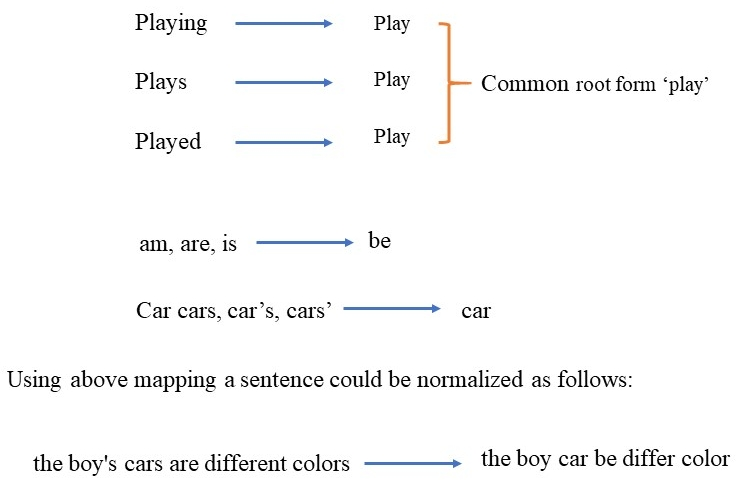
\includegraphics[width=11cm]{assets/stemming.jpg}
	\caption{Words stemming. \\ \url{www.datacamp.com/community/tutorials/stemming-lemmatization-python}.}
	\label{fig:stemming}
\end{figure}

Con questa tecnica è possibile ridurre il numero di tokens, dal momento che le stesse parole con suffisso diverso verranno mappate nella medesima radice. Inoltre non è necessario che una parola dopo il processo di stemming venga trasformata in un'altra di senso compiuto, quello che conta è la semantica del token.


\subsubsection{Vector encoding}

L'insieme delle parole ottenute costituisce il dizionario del corpora. Si procede costruendo una matrice booleana composta dai tweets sulle righe e le parole del dizionario sulle colonne.\\

Sia $D = \{w_1,\ w_2, ...,\ w_m\}$ il dizionario individuato dall'insieme delle $n$ parole univoche.

Sia $T_i = \{t_{i0}\ ,t_{i1},\ ...,\ t_{ik}\}, \ 1 \leq i \leq n$ l'i-esimo tweet composto da $k$ tokens opportunamente stemmatizzati.\\

Viene definita la matrice $M_{n,m}$
\[
M[i,j] =
\begin{cases}
1 & \text{se}\ w_j \in T_i\\
0 & \text{altrimenti}
\end{cases}
\ t.c\ 1\leq i\leq n,\ 1 \leq j \leq m
\]


\subsection{Rappresentazione mediante transformer}


\subsubsection{BERT}

\subsubsection{Sentence-BERT}


\section{Caratteristiche linguistiche}
La scelta di features ad alto contenuto informativo ed indipendenti tra loro, è un passo fondamentale per un corretto riconoscimento di pattern nei dati.
A questo scopo vengono estratte delle caratteristiche linguistiche dal testo che sono rilevanti per il riconoscimento dell'ironia. Più le caratteristiche sono discriminanti quando si esprime un messaggio ironico, meglio si potranno distinguere le due classi. Queste features, insieme alla codifica testuale, verranno usate per creare il modello.

\subsection{PP (Pragmatic particles)}
Per catturare il senso non letterale racchiuso in ogni messaggio, vengono considerati alcuni elementi linguistici di seguito elencati.

\subsubsection{Emoticons}
Le emoticons sono riproduzioni stilizzate di quelle principali espressioni facciali umane che esprimono un'emozione. In accordo con l'assunzione che esista una relazione tra il sentimento espresso e l'ironia, queste vengono distinte in due categorie:
\begin{itemize}
	\item
	Positive
	
	E.g.: ':-)', ':-D'
	\item
	Negative
	
	E.g.: ':-(', ':=('
	
\end{itemize}

\subsubsection{Acronimi}
Gli acronimi sono un ulteriore strumento della comunicazione non verbale. Come le emoticons vengono presi in considerazione dal momento che possono esprire sentimenti positivi o negativi, infatti possiamo anch'essi dividerli in due categoire:

\begin{itemize}
	\item
	Positivi
	
	E.g.: 'ROLF' (Rolling On Floor Laughing), 'LHO' (Laughing Head Off)
	\item
	Negativi
	
	E.g: 'BM' (Bad Manner)
	
\end{itemize}

\subsubsection{Espressioni onomatopeiche}
L'uso di espressioni onomatopeiche come 'boom' o 'clap' possono essere utilizzate nell'esprimere un messaggio ironico. Tuttavia in questo caso viene presa in considerazione solo la frequenza di queste espressioni, al contrario di come visto in precedenza per le emoticons e gli acronimi, dove si valutava anche la polarità.

\subsubsection{Punteggiatura}
La punteggiatura nei social media non segue le convenzioni ortografiche:\\
E.g.: 'Do you hear us now ?????'\\
Per questa ragione viene contata la frequenza di virgole, punti di domanda e punti esclamativi.

\subsubsection{Estrazione particelle pragmatiche}
Di seguite viene mostrato un esempio di come le particelle pragmatiche vengono estratte da un messaggio:

\begin{lstlisting}[caption={Esempio di tweet processato per estrarre le particelle pragmatiche.}]
Tweet: ':D lmao! RT @KarlDetkenProDJ iPad Humor Steve, I'ma let you finish,
        but Moses had the greatest  tablet of all time ;) clap clap'
Emot (-, +)  >>> [0, 1]
Init (-, +)  >>> [0, 1]
Onom (#)     >>> [2]
Punct        >>> {',': 2, '!': 1, '?': 0}
\end{lstlisting}


\subsection{POS (Part Of Speech)}
La struttura delle frasi che costituiscono il tweet, può essere un indicatore per il riconoscimento dell'ironia. A questo scopo viene tenuta in considerazione la frequenza dei POS (part-of-speech) tag relativi ai tokens parole presenti in un messaggi.

Per associare i POS tag ad ogni tweet viene utilizzato un POS tagger\footnote{ARK Twitter Part-of-Speech Tagger: \url{www.ark.cs.cmu.edu/TweetNLP/}} supervisionato specifico per il dominio considerato. Si procede con una tokenizzazione del tweet per poi associare ad ognuno di questi il corretto tag. Di seguito la lista di tags considerati:\\


\begin{varwidth}[t]{\textwidth}
	\textbf{Nominale}
	\begin{itemize}
		\item \textbf{N}: Nome comune
		\item \textbf{O}: Pronome personale
		\item \textbf{\^}: Nome proprio
		\item \textbf{S}: Nominale + Possessiva
		\item \textbf{Z}: Nome proprio + Possessiva
	\end{itemize}
\end{varwidth}
\hspace{4em}
\begin{varwidth}[t]{\textwidth}
	\textbf{Closed-class words}
	\begin{itemize}
		\item \textbf{D}: Determiner
		\item \textbf{P}: Pre/Post-posizione;\\Congiunzione subordinante
		\item \textbf{\&}: Congiunzione coordinante
		\item \textbf{T}: Verb particles
		\item \textbf{X}: Existential there
	\end{itemize}
\end{varwidth}\\\\

\begin{varwidth}[t]{\textwidth}
	\textbf{Open-class words}
	\begin{itemize}
		\item \textbf{V}: Verbo
		\item \textbf{A}: Aggettivo
		\item \textbf{R}: Avverbio
		\item \textbf{!}: Interjection
	\end{itemize}
\end{varwidth}
\hspace{11em}
\begin{varwidth}[t]{\textwidth}
	\textbf{Composti}
	\begin{itemize}
		\item \textbf{L}: Nominale + Verbo (e.g.: I'm)
		\item \textbf{M}: Nome proprio + Verbo
		\item \textbf{Y}: X + Verbo
	\end{itemize}
\end{varwidth}\\\\\\\\
Di seguito è mostrato un esempio di POS tags associati al tweet passando per i tokens:


\begin{lstlisting}[caption={Esempio di tweet con POS tag associte.}]

Tweet: 'Need a second opinion? Who gave you the first one?'
Tokens  >>> [Need], [a], [second], [opinion], [?], [Who],
            [gave], [you], [the], [first], [one], [?]
Tags    >>> ['V', 'D', 'A', 'N', ',', 'O', 'V', 'O', 'D', 'A', '$', ',']
Freq.   >>> {'N': 1, 'O': 2, '^': 0, 'S': 0, 'Z': 0, 'V': 2,
             'A': 2, 'R': 0, '!': 0, 'D': 2, 'P': 0, '&': 0,
             'T': 0, 'X': 0, 'L': 0, 'M': 0, 'Y': 0}
\end{lstlisting}
Come si può notare, il POS tagger associa dei tag che non sono stati elencati sopra, i verranno semplicemente ignorati e non utilizzati come features per il modello. 

\subsection{EMOT (Emotional Features)}
Alcune teorie psicologiche suggeriscono l'esistenza di emozioni primarie. Per questo motivo sono stati utilizzati i lessici EmoLex e EmoSenticNet, in cui vengono riportate le sfere emotive a cui appartengono le parole.
I lessici si possono intendere come diversi insiemi che caratterizzano le emozioni primarie, dove ognuno di questi insiemi è composto dalle parole che sono considerate appartenenti a quella specifica categoria emozionale. Inoltre gli insiemi considerati non devono necessariamente essere disgiunti.\\
Qualche esempio di seguito:

$birthday \in JOY \land birthday \in SURPRISE \land birthday \in ANTICIPATION$

$honor \in TRUST$

$ stair \notin (JOY \cup SURPRISE \cup ANTICIPATION \cup TRUST) $\\


Come feature aggiuntiva per il riconoscimento dell'ironia, dato un tweet si considerano tutti i tokens validi che rappresentano le parole. Quindi si procede consultando i lessici per ognuna delle parole, così da recuperate le sfere emotive a cui è essa associata. Una volta eseguita l'operazione per tutte queste, si calcola la frequenza totale di ogni emozione all'interno del tweet.

Le due risorse si basano su differenti teorie che identificano ognuna le proprie emozioni primarie, per questo motivo si combina il risultato di entrambe sommando le frequenze ottenute da ognuna delle due risorse.

\begin{table}[h!]
	\centering
	\begin{tabular}[t]{l|l}
		\hline
		\textbf{Emozione} & \textbf{Lessico} \\
		\hline
		Anger			& EmoLex, EmoSenticNet \\
		Anticipation	& EmoLex \\
		Disgust			& EmoLex, EmoSenticNet \\
		Fear			& EmoLex, EmoSenticNet \\
		Joy				& EmoLex, EmoSenticNet \\
		Sadness			& EmoLex, EmoSenticNet \\
		Suprise			& EmoLex, EmoSenticNet \\
		Trust			& EmoLex \\
		\hline
	\end{tabular}
	\caption{Emozioni primarie dei lessici.}
\end{table}


Un esempio di come vengono estratte le features emozionali da un tweet:

\begin{lstlisting}[caption={Esempio di estrazione delle emozioni da un tweet.}]

Tweet: 'I nominate @MrsStephenFry for a Shorty Award in because... why
        not? http://bit.ly/shorty'
Words	     >>> ['nominate', 'shorty', 'award']
EmoLex       >>> {'anger': 0, 'anticipation': 1, 'disgust': 0, 'fear': 0,
                  'joy': 1, 'sadness': 0, 'surprise': 1, 'trust': 1}
EmoSenticNet >>> {'anger': 0, 'disgust': 0, 'joy': 3, 'sadness': 0,
                  'surprise': 0, 'fear': 0}
Combined     >>> {'sadness': 0, 'anticipation': 1, 'fear': 0, 'anger': 0,
                  'joy': 4, 'disgust': 0, 'trust': 1, 'surprise': 1}
\end{lstlisting}

\section{Modelli supervisionati}
Il machine learning è lo studio di algoritmi che migliorano automaticamente attraverso l'esperienza, ed è sottoinsieme dell'intelligenza artificiale. Il machine learning crea modelli matematici basati sui dati, i quali vengono utilizzati per far apprendere alla macchina, con lo scopo di fare previsioni o decidere riguardo dati che non sono mai stati visti prima.


\begin{figure}[!h]
	\centering
	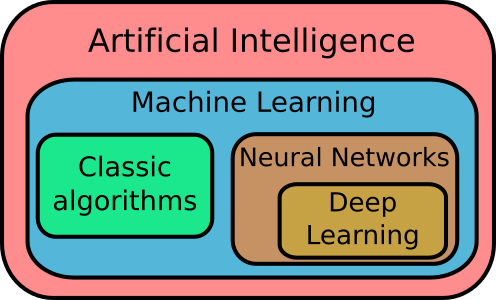
\includegraphics[width=7cm]{assets/ai_diagram.png}
	\caption{Diagramma intelligenza artificiale. \\ \url{https://mc.ai/machine-learning-in-5-minutes/}.}
	\label{fig:artificial-intelligence}
\end{figure}

Nello specifico i modelli supervisionati fanno parte di quell'insieme di algoritmi "classici" che per apprendere dai dati ed estrarre dei pattern da questi, oltre ai dati di training in input, hanno bisogno delle relative etichette. Questa informazione aggiuntiva viene usata nella fase di apprendimento e indica a priori la relativa classe di appartenenza delle istanze che compongono il dataset. Nel caso dell'ironia si fa riferimento ad algoritmi supervisionati di machine learning per risolvere un problema di classificazione, ovvero dato un tweet classificarlo come "ironico" o "non ironico".

Esistono diversi algoritmi per creare modelli supervisionati, quelli che sono stati utilizzati negli esperimenti sono:
	\begin{itemize}
	\item Decision Tree
	\item Multinomial Naive Bayes
	\item Bayesian Network
	\item Support Vector Machine
\end{itemize}

\subsection{Decision Tree}
Un albero di decisione è un modello predittivo con una struttura ad albero. Ogni nodo interno rappresenta una feature, un arco verso un nodo figlio rappresenta un possibile valore per quella proprietà, ovvero una decisione, e una foglia il valore predetto. Il processo consiste in una sequenza di test, comincia sempre dal nodo radice, e procede verso il basso. A seconda dei valori rilevati in ciascun nodo, si otterrà un path che porterà ad un nodo foglia e quindi una classificazione.

\begin{figure}[!h]
	\centering
	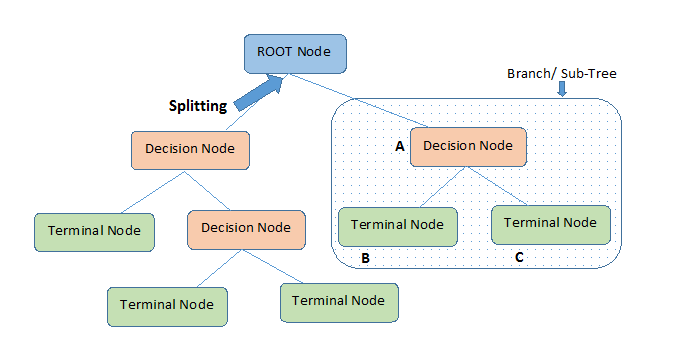
\includegraphics[width=13cm]{assets/decision_tree.png}
	\caption{Albero di decisione. \\ \url{www.medium.com/datadriveninvestor/decision-tree-algorithm}.}
	\label{fig:decision-tree}
\end{figure}

Gli alberi di decisione hanno il vantaggio della semplicità. Infatti è possibile seguire il percorso radice-foglia per analizzare come la macchina è giunta a una determinata decisione basandosi sui dati in input. Questo processo rappresenta di fatto la logica utilizzata dalla macchina per interpretare i dati.

Un problema degli alberi di decisione è che tendono ad andare in overfitting.


\subsection{Naive Bayes}
L'algoritmo di classificazione Naive Bayes si basa sull'applicazione del teorema di Bayes:
$$P(A|B) = \frac{P(B|A)P(A)}{P(B)}$$
Contestualizzato per la creazione di un modello per un task di classificazione, si ha la tupla composta dalle features di un particolare documento identificato da:

$$\textbf{X} = (x_1, x_2, ..., x_n)$$
Applicando il teorema di Bayes, rappresentando $y$ come classe di appartenenza per un individuo si ottiene:

$$P(y|\textbf{X}) =
\frac{P(\textbf{X}|y)P(y)}{P(\textbf{X})}$$
Si noti che la parte destra dell'uguaglianza è la probabilità a priori, ed è stimabile utilizzando il dataset a disposizione. In questo modo è possibile calcolare la probabilità a posteriori. Il classificatore preso in questione è considerato "naive", in quanto si assume che le features siano indipendenti. Con questa assunzione si procede sviluppando l'equazione:
$$P(y|x_1, x_2, ..., x_n) =
\frac
	{P(x_1|y)P(x_2|y)...P(x_n|y)P(y)}
	{P(x_1)P(x_2)...P(x_n)}$$
A questo punto, date le features di un individuo, è possibile calcolare la probabilità che questo appartenga ad una particolare classe $y$. Inoltre, fissate le fetures, il denominatore è costante. Si considera quindi:
$$P(y|x_1, x_2, ..., x_n) \propto
P(y)\prod\limits_{i=1}^{n}P(x_i|y)
$$
Un individuo viene classificato come quella classe $y$ che massimizza la probabilità a posteriori:
$$\hat{y} = \argmax_y P(y)\prod\limits_{i=1}^{n}P(x_i|y)$$


\subsection{Multinomial Naive Bayes}
Nell'algoritmo Naive Bayes, avendo dati n-dimensionali e k classi, la probabilità a posteriori si ottiene conoscendo $P(x_i|y_j)$ per ogni $1\leq n,\ 1\leq j \leq k$

Queste probabilità vanno stimate dal dataset, e nella variante Multinomial Naive Bayes si considera una distribuzione multinomiale per ognuna di esse. Si hanno quindi i parametri $\theta_y = (\theta_{y1}, \theta_{y2}, ...\theta_{yn})$, dove $\theta_{yi} = P(x_i|y)$ e vengono stimati in questo modo:

$$\hat{\theta}_{yi} = \frac{N_{yi} + \alpha }{N_{y} + \alpha n}$$
Dove $N_{yi} = \sum_{x \in T}x_i$ è il numero di volte che, nel training set $T$, la feature $i$ appartiene alla classe $y$, e $N_{y} = \sum_{i=1}^{n}N_{yi}$.

The smoothing priors $\alpha \geq 0$ accounts for features not present in the learning samples and prevents zero probabilities in further computations. Setting $\alpha = 1$ is called Laplace smoothing, while $\alpha < 1$ is called Lidstone smoothing.


\subsection{Bayesian Network}
I classificatori naive Bayes si basano sull'assunzione di indipendenza delle caratteristiche. Ciò permette di semplificare 
\subsection{Support Vector Machine}


\section{Strumenti utilizzati}
\subsection{Scikit-learn}
\subsection{Weka}




\chapter{Campagna sperimentale}

\section{Dataset}
Fare notare che è in inglese

Trattandosi di un modello supervisionato, è richiesto che il dataset sia etichettato. Per associare una specifica label ai messaggi generati dagli utenti si possono seguire due strade:

\begin{itemize}
	\item \textbf{Self-Tagging}:
	\label{chap:self-taggin}
	Twitter mette a disposizione l'utilizzo degli hashtag nei messaggi. Assumendo che un utente utilizzi l'hashtag \emph{\#irony} con la volontà di esprimere ironia, è facile collezionare una serie di tweet etichettati come ironici.
	
	\item \textbf{Crowdsourcing}:	
	I vari tweet vengono etichettati manualmente da alcune persone
\end{itemize}

Nel caso specifico, viene utilizzato il dataset \emph{TwReyes2013}, composto da 40,000 tweet in lingua inglese, accumulati usando la tecnica self-tagging. Vengono quindi considerati 4 hashtag diversi:


\begin{table}[ht]
	\centering
	\begin{tabular}[t]{llr}
		\hline
		\textbf{Numero} & \textbf{Hashtag}  & \textbf{Label assocaita}\\
		\hline
		10,000 & \emph{\#irony}     & ironico     \\
		10,000 & \emph{\#education} & non ironico \\
		10,000 & \emph{\#humor}     & non ironico \\
		10,000 & \emph{\#politics}  & non ironico \\
		\hline
	\end{tabular}
	\caption{Hashtag e label associate}
\end{table}%

\section{10-Folds Cross-Validation}
Per la fase di training dei modelli è necessario suddividere il dataset a disposizione in due diversi insiemi: training-set e test-set. Questo è un passaggio fondamentale in quanto non si otterrebbero delle misure di performance valide testando i modelli su dati che sono stati utilizzati per la fase di trainig. In pratica si vuole testare il modello su dati che non sono mai stati visti in precedenza.

Prima di iniziare la fase ti training, i dati in input, che sono composti dalla matrice contenente le features estratte, vengono opportunamente mescolati. Con questo si intende che le righe della matrice vengono casualmente cambiate di posto, chiaramente mantenendo coerenza con le labels associate. Un aspetto importante è che lo shuffle della matrice è eseguito con lo stesso seed per tutti i modelli, così da ottenere delle misure di performance statisticamente valide.

Le performance ottenute, dipendono anche da come è stato diviso il dataset tra training-set e test-set. Per questo motivo viene utilizzata la tecnica k-Folds Cross-Validitation, che permette di sfruttare diverse porzioni di dati per i due insiemi. Il vantaggio di questa tecnica è quello di ottenere valutazioni più affidabile mediando i risultati di ognuno dei k modelli di cui è stato fatto il training, a discapito del tempo necessario, in quanto si effettuerà k volte il training di un modello.

Per gli esperimenti effettuati, è stato scelto $k=10$, ovvero il dataset è stato diviso 10 volte, utilizzando ad ogni iterazioni una porzione di dati diversa per il trainig-set e test-set. Avendo scelto questo valore di $k$, la proporzione tra i due insiemi sarà sempre $90\%$ per il training-set e $10\%$ per il test-set.

Nel seguente diagramma si possono considerare i pallini verdi e rossi come i tweets ironici e non ironici. Quindi, fissata un'istanza del dataset mescolato, si considera una sliding window di dimensione $\#samples \cdot \frac{1}{k}$, dove per ogni $k$ iterazione viene effettuato il training di un nuovo modello.

\begin{figure}[!h]
	\centering
	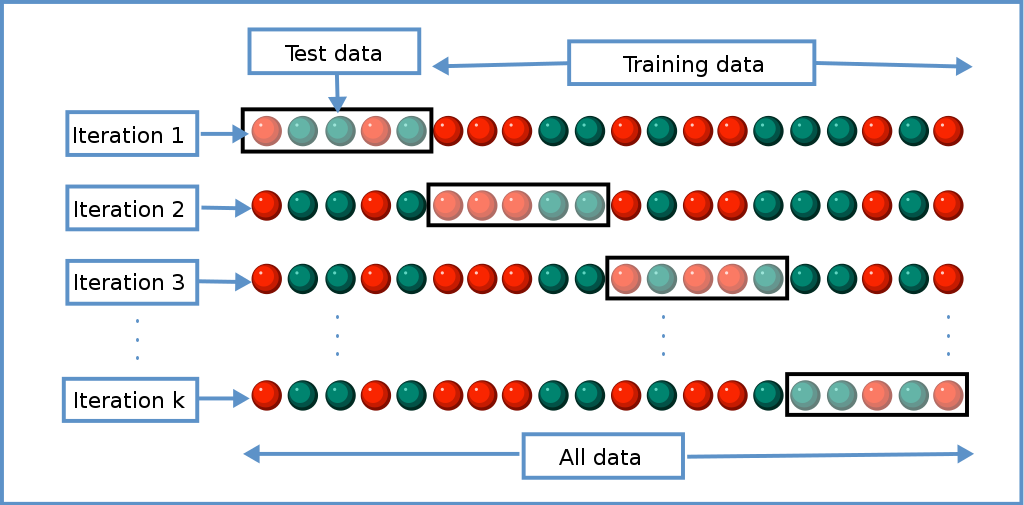
\includegraphics[width=13cm]{assets/cross-validation.png}
	\caption{k-Folds Cross-Validation. \\ \url{www.wikipedia.org/wiki/Cross-validation_(statistics)}.}
	\label{fig:cross-validation}
\end{figure}


\section{Misure di performance}
Essendo stati creati diversi modelli, è necessario valutarli. Avendo diviso il dataset a disposizione tra test-set e training-set, una volta completata la fase di training è possibile utilizzare il test-set per la valutazione. Si procede prendendo un tweet e facendolo classificare al modello, il quale verrà quindi identificato come ironico o non ironico. Trattandosi di modelli supervisionati, oltre ai dati si hanno a disposizione le labels associate, è quindi possibile confrontare l'output fornito dal modello con la reale classe di un tweet. Da qui si può capire se per quel particolare individuo, la classificazione è corretta o meno.

Per la valutazione si utilizza tutto il test-set a disposizione e viene contano il numero di:
\begin{itemize}
	\item \textbf{TP} (True positive): Un tweet ironico è classificato come ironico - \emph{corretto}
	
	\item \textbf{TN} (True negative): Un tweet non ironico è classificato come non ironico - \emph{corretto}
	
	\item \textbf{FP} (False positive):	Un tweet non ironico è classificato come ironico - \emph{errato}
	
	\item \textbf{FN} (False negative):	Un tweet ironico è classificato come non ironico - \emph{errato}
\end{itemize}
Si noti che un modello può sbagliare la classificazione in due modi diversi, e c'è differenza tra classificare un tweet ironico come non ironico piuttosto che uno non ironico come ironico. Questi valori verranno poi analizzati sfruttando una matrice di confusione:

\begin{figure}[!h]
	\centering
	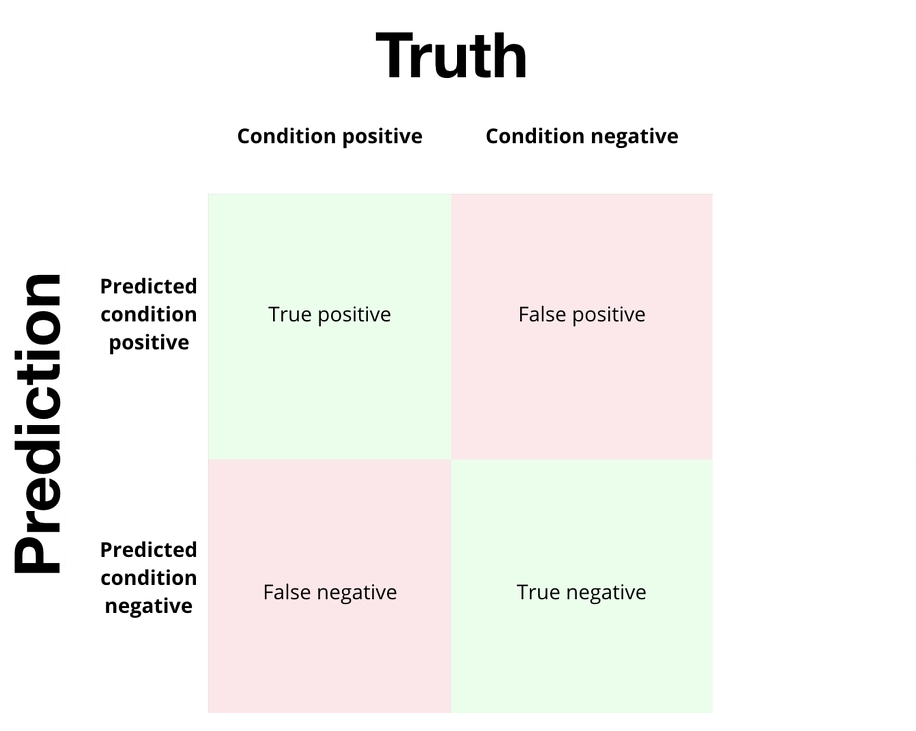
\includegraphics[width=10cm]{assets/confusion-matrix.jpg}
	\caption{Confusion matrix. \url{www.radiopaedia.org/cases/confusion-matrix-3}.}
	\label{fig:decision-tree}
\end{figure}

Basandosi su questi dati vengono definite delle misure di performance per la valutazione:

\begin{itemize}
	\item \textbf{Accuracy}: Il rapporto tra il numero di classificazioni corrette e le classificazioni totali.
	
	$$Accuracy = \frac{TP + TN}{TP + FP + TN + FN} $$
	
	\item \textbf{Precision}: La porizione di classificazioni positive corrette.
	
	$$Precision = \frac{TP}{TP + FP} $$
		
	\item \textbf{Recall}: La porzione di sample positivi identificati.
	$$Recall = \frac{TP}{TP + FN} $$
	
	
	\item \textbf{F-measure}: Metrica per calcolare la valutazione complessiva. Formalmente è definita come la media armonica di recall e precision.
	$$F\text{-}measure =  2 \cdot \frac{Precision \cdot Recall}{Precision + Recall} $$
	
\end{itemize}

\section{Esperimenti}

\subsection{Caratteristiche linguistiche}
\subsection{BOW + Caratteristiche linguistiche}
\subsection{BERT + Caratteristiche linguistiche}
\subsection{Sentence-BERT + Caratteristiche linguistiche}
\subsection{BOW vs BERT vs Sentence-BERT}
\subsection{Analisi lessico con PCA}


\chapter{Conclusioni e sviluppi futuri}


\end{document}


TESI: 
- Introduzione (3 pagine)
- Descrizione problema
Comprensibile
Social network prodotto linguaggio naturale caratterizzato da ironia ed è importante saperla distinguure e il motivo.
- Come ho affronatato
Tenciche di NLP e problema di apprendiamento automatico usando machine learnign
- Sintesi risultati
- Struttura della tesi
- Capitolo 1 -> Stato dell'arte
1.1 approcci supervisoonati
1.2 non supervisionati
1.3 semi supervisionati
- Captiolo 2 -> Ssitema realizzato		
2.1 Descrizione del sitema proposto
Workflow e descrizione di massima del sistema
2.2 Rappresentazione del testo
2.2.1 Rappresentazione booleana
2.2.2 Rappresentazione mediante transformer
2.3 Caratteristiche linguistiche
2.3.1 POS
2.3.2 PP
2.3.3 Emot			
2.4 Modelli supervisionati
2.4.1 Alberi di decisione
ecc...
2.5 Strumenti utilizzati
2.5.1 SKleanr
2.5.2 Weka

- Capitolo 3 -> Campagna sperimetnale
3.0 Dataset e misure di performance
3.1 Rappresentazione BOW + caratteristiche linguistiche
3.2 Rappresentazione BERT + caratteristiche linguistiche
3.3 Analisi lessico con PCA
- Capitolo 4 -> Conlcusioni e sviluppi futuri
